\documentclass[conference]{IEEEtran}
\IEEEoverridecommandlockouts
% The preceding line is only needed to identify funding in the first footnote. If that is unneeded, please comment it out.
\usepackage{cite}
\usepackage{amsmath,amssymb,amsfonts}
\usepackage{algorithmic}
\usepackage{graphicx}
\usepackage{textcomp}
\usepackage{xcolor}
\def\BibTeX{{\rm B\kern-.05em{\sc i\kern-.025em b}\kern-.08em
  T\kern-.1667em\lower.7ex\hbox{E}\kern-.125emX}}
\begin{document}

\title{Risk-Neutral Pricing Model of Uniswap Liquidity Providing Position: A Stopping Time Approach\\}

\author{\IEEEauthorblockN{HOU Liang}
\IEEEauthorblockA{\textit{Antalpha labs} \\
\textit{Antalpha}\\
Beijing, China \\
liang.hou@antalpha.com}
\and
\IEEEauthorblockN{YU Hao}
\IEEEauthorblockA{\textit{Antalpha labs} \\
\textit{Antalpha}\\
Hangzhou, China \\
yuhao0126liuer@gmail.com}
\and
\IEEEauthorblockN{XU Guosong}
\IEEEauthorblockA{\textit{Derivatives Trading Division} \\
\textit{China Merchants Securities Co., Ltd.}\\
Shenzhen, China \\
xuguosong@cmschina.com.cn}
}

\maketitle

\begin{abstract}
In this paper, we introduce a novel pricing model for Uniswap V3, built upon stochastic processes and the Martingale Stopping Theorem. This model innovatively frames the valuation of positions within Uniswap V3. We further conduct a numerical analysis and examine the sensitivities through Greek risk measures to elucidate the model's implications. The results underscore the model’s significant academic contribution and its practical applicability for Uniswap liquidity providers (LPs), particularly in assessing risk exposure and guiding hedging strategies.
\end{abstract}

\begin{IEEEkeywords}
Uniswap, pricing model, greeks, perpetual option, risk management, hedging strategies
\end{IEEEkeywords}

\section{Introduction}
Uniswap\cite{b1}, launched in November 2018, represents a decentralized, open-source protocol for cryptocurrency exchange. As the first automated market maker (AMM) to achieve widespread adoption, Uniswap enables users to conduct token swaps directly from their wallets via liquidity pools. In these pools, liquidity providers (LPs) earn fees by contributing their assets.

The introduction of Uniswap V3 brought significant advancements, most notably the concept of concentrated liquidity. This feature allows LPs to allocate their capital to specific price ranges, enhancing capital efficiency and yielding higher returns while simultaneously mitigating price risk. Furthermore, Uniswap v3 incorporates multiple fee tiers, thereby providing LPs with flexibility in selecting their compensation levels in accordance with their risk tolerance.

With the ongoing expansion of decentralized finance (DeFi) adoption, the demands on LPs in Uniswap v3 have intensified. LPs are now required to meticulously balance a myriad of factors, including risk, returns, and volatility, necessitating a sophisticated understanding and strategic approach to liquidity provision.


\section{Related Work and Limitations}

\subsection{Loss-Versus-Rebalancing (LVR)}

LVR is a metric designed to quantify the impact of adverse selection on automated market maker (AMM) LPs\cite{b2}. LVR captures the costs incurred by LPs due to stale prices that better-informed arbitrageurs exploit. Unlike impermanent loss, which only considers the starting and ending points of a trade, LVR compares the performance of LPs to a rebalancing portfolio, highlighting additional costs associated with providing liquidity.

LVR incorporates volatility into its calculations, making it a useful tool for selecting the optimal liquidity pool. However, it remains primarily a risk assessment tool. It does not evaluate the returns for LPs when exiting positions at different prices, nor does it provide guidance on the optimal range for market-making activities.

\subsection{Guillaume Lambert}
Guillaume Lambert focused on pricing within the Black-Scholes-Merton (BSM) framework in his work\cite{b3}\cite{b4}. He viewed liquidity positions as perpetual options and attempted to replicate liquidity positions with covered calls. He also extends his model towards implied volatility and hedging. However, a limitation of Lambert's model is the specification of an expiration time T, which inherently makes it an approximation rather than a precise solution. Additionally, Lambert explored the use of stochastic processes to calculate the probability of prices remaining within a position range, which has greatly inspired our research. We aim to build upon this foundation by starting from stochastic processes to initiate our study.

\subsection{Martingale and first hitting problem with two boundaries}
Unlike traditional derivatives with specific expiration dates, Uniswap V3 contracts are perpetual, persisting until the price breaches predefined boundaries or the contract holder voluntarily ceases market-making. In scenarios where the price crosses these preset boundaries, this constitutes a classic First Passage Problem, for which Darling and Siegert provided a derivation of the stopping time distribution using the Laplace Transform in 1953\ \cite{b5}. We have further discovered that the expected value of the payoff under the risk-neutral measure contains exclusively terms of the form $\tau^n \exp(-r\tau)$  which are associated with the stopping time $\tau$. Therefore, we employ the Laplace Transform and its implications to derive the present value when the holder does not elect to terminate prematurely. In situations where the contract holder actively ceases market-making, we draw inspiration from the pricing methodology for Perpetual American Puts described by Shreve (2004) \cite{b6} and use numerical optimization to determine the optimal stopping strategy.

\section{Derivation}

\subsection{Summary of Model Derivation}

% 在这里增加公式

Uniswap V3 can be divided into two primary pricing components: the Liquidity Provider (LP) segment and the Rebate segment. The LP component is structured to accommodate either European or American option styles. Under the European construct, the Uniswap contract realizes its terminal value solely upon the price breaching the predetermined upper or lower thresholds. In contrast, the American framework allows the contract holder the flexibility to terminate the automated market-making process at any chosen point in time.
The valuation of the Rebate segment hinges on the method selected by the contract holder for Rebate withdrawal. The upper limit scenario assumes the possibility of continuous Rebate extraction at the precise point of accrual. Meanwhile, the lower limit approach considers a singular, comprehensive withdrawal of all Rebates coinciding with the termination of the contract.

\subsection{Divide and Conquer}\label{AA}
We initially assume that the ETHUSDT price follows a Geometric Brownian Motion (GBM) characterized by drift $\mu$ and annualized volatility $\sigma$ :
$$dS(t)=\mu S(t)dt+ \sigma S(t)dB_t$$
or alternatively:
$$
S(t) = S_0\exp((\mu-\frac{\sigma^2}{2})t+\sigma B_t)
$$
Define the unit price of ETHUSDT as follows
$$P(t) = \frac{S(t)}{S_0}=\exp((\mu-\frac{\sigma^2}{2})t+\sigma B_t)$$
We partition the pricing structure of Uniswap V3 into two segments:
$$
V = V_{\text{LP}}+V_{\text{fee}}
$$
\subsubsection{Liquidity Provider segment}
The unit price of the LP segment within the Uniswap V3 Contract, constrained by $S_H>S_0> S_L$, can be expressed as:
$$
\begin{aligned}
V_\text{LP}(P_t)&=
\begin{cases}
L_q P(t)(\frac{1}{\sqrt{L}}-\frac{1}{\sqrt{H}}), P(t)<L \\
L_q(2\sqrt{P(t)}-\sqrt{L}-\frac{P(t)}{\sqrt{H}}), L<P(t)<H \\
L_q(\sqrt{H}-\sqrt{L}), H<P(t)
\end{cases} \\
\end{aligned}
$$
where $H, L$ represent the unit bounds:
$$
\begin{aligned}
H &= \frac{S_H}{S_0}\\
L &= \frac{S_L}{S_0}\\
\end{aligned}
$$
Additionally, the Liquidity Parameter is defined as:
$$
L_q =\frac{1}{2-\sqrt{L}-\frac{1}{\sqrt{H}}}
$$
\subsubsection{Rebate segment}
% 两个版本
The formulation for the rebate fee segment is comparatively straightforward:
$$
V_{\text{fee}} = C_a L_q t=365\times C_d L_q t
$$
where $C_a, C_d$ are the daily and annual rebate rate.
\subsection{European LP Pricing}\label{AA}
% assumption 
We are interested in evaluating:
$$
V(0) = \mathbb E(V(t)) = \mathbb E(V_{\text{LP}}(t))+\mathbb E(V_{\text{fee}}(t))
$$
For the Uniswap V3 opsition, the stopping time $\tau$ is defined as:
$$\tau = \inf\limits_{t<\infty}\{S(t)\leq S_L \text{ or }S(t)\geq S_H\}$$
If the contract cannot be terminated before the stopping time, the current valuation of Uniswap V3 can be formulated as:
$$
\begin{aligned}
V_{E}(0) &= \mathbb E(V(t))\\
&= \mathbb E(V_{\text{LP}}(t))+\mathbb E(V_{\text{fee}}(t))\\
&= \mathbb E[e^{-r\tau}\text{LP}_{ H}|S(\tau)=S_H]+ \mathbb E[e^{-r\tau}\text{LP}_{ L}|S(\tau)=S_L] \\& \mathbb +E(V_{\text{fee}}(t))\\
&= \text{LP}_{H} \mathbb E[e^{-r\tau}|S(\tau)=S_H]+\text{LP}_{L} \mathbb E[e^{-r\tau}|S(\tau)=S_L] \\
&+\mathbb E(V_{\text{fee}}(t))
\end{aligned}
$$
The normalized log-unit price process of ETHUSDT is given by:
$$
\bar W(t) = \frac{\ln P(t)}{\sigma}=(\frac{\mu}{\sigma}-\frac{\sigma}{2})t + B_t
$$
Let us denote:
$$
\mu' = \frac{\mu}{\sigma}-\frac{\sigma}{2}
$$
Thus, we have:
$$
\bar W(t) =x +\mu't +B_t
$$
where $x$ is the start point, $a,b$ are designated as the unit bounds:
$$
\begin{aligned}
b &= \frac{\ln H}{\sigma}, b' = b-x\\
a &= \frac{\ln L}{\sigma}, a' = x-a\\
\end{aligned}
$$
Moreover, it also holds that:
$$\tau = \inf\limits_{t<\infty}\{\bar W(t)\leq a \text{ or }\bar W(t)\geq b\}$$
Utilizing the Laplace Transform, we can express the following expectations:
$$
\mathbb E[e^{-r\tau}|S(\tau)=S_H] = \exp({\mu'b'})\frac{\sinh[a'\sqrt{\mu'^2+2r}]}{\sinh[(b-a)\sqrt{\mu'^2+2r}]}
$$
$$
\mathbb E[e^{-r\tau}|S(\tau)=S_L]=\exp({-\mu'a'})\frac{\sinh[(b'\sqrt{\mu'^2+2r}]}{\sinh[(b-a)\sqrt{\mu'^2+2r}]}
$$
\subsection{American LP Pricing}
In Euro-like pricing, liquidity providers can only exit when the price reaches the boundary. We further propose an American-like pricing model that allows liquidity providers to exit at any time.
As Uniswap V3 contracts are perpetual, the termination of the contract relies exclusively on price movements, independent of time $t$. Therefore, it can be assumed that there exist boundaries determined solely by price levels. This implies that exit strategies should be based only on price considerations, analogous to the derivation of the perpetual American put option in Shreve's work\cite{b6}. So we have:
$$
L<L_1<x<L_2<H
$$
where terminating automated market-making at prices 
$L_1$ or $L_2$. A set of stopping boundaries $L_1, L_2$ can be determined through numerical optimization.
First, we denote $c,d$ as previous section:
$$
\begin{aligned}
d &= \frac{\ln L_2}{\sigma}, d' = d-x\\
c &= \frac{\ln L_1}{\sigma}, c' = x-c\\
\end{aligned}
$$
Then the equivalent price of the European contract:
$$
\begin{aligned}
V_E &= LP_{L_2} \exp({\mu'd'})\frac{\sinh[c'\sqrt{\mu'^2+2r}]}{\sinh[(d-c)\sqrt{\mu'^2+2r}]}\\
&+LP_{L_1}\exp({-\mu'c'})\frac{\sinh[(d'\sqrt{\mu'^2+2r}]}{\sinh[(d-c)\sqrt{\mu'^2+2r}]}    
\end{aligned} 
$$
The American contract can be priced using optimization techniques as following:

$$
V_A = \mathop{\max_{L<L_1<x<L_2<H}V_E(L_1,L_2)}
$$

\subsection{Rebate Pricing}
For the rebate segment, if we assume that we can withdraw rebates continuously,(it is an upper bound of rebate)
$$
\begin{aligned}
\mathbb E(V_{\text{fee}}(t)) & =\mathbb{E}\left[\int_0^\tau C_aL_q \cdot e^{-r t} d t\right] \\
& =C_aL_q \cdot \mathbb{E}\left[\int_0^\tau e^{-r t} d t\right] \\
& =C_aL_q \cdot \mathbb{E}\left[\frac{1-e^{-r \tau}}{r}\right] \\
& =\frac{C_aL_q}{r} \cdot (1-\mathbb{E}\left[{e^{-r \tau}}\right])
\end{aligned}
$$
where,
$$
\begin{aligned}
&\mathbb{E} [e^{-r \tau}]:=F(r)\\
&=\frac{e^{-\mu'a'} \operatorname{sh}\left(b' \sqrt{2 r+\mu'^2}\right)+e^{\mu' b'} \operatorname{sh}\left(a' \sqrt{2 r+\mu'^2}\right)}{\operatorname{sh}\left((b-a) \sqrt{2 r+\mu'^2}\right)}
\end{aligned}
$$
For the lower bound, we assume that we can withdraw all rebates when LPs close their position,
$$
\mathbb E(V_{\text{fee}}(t)) = \mathbb E(C_aL_qe^{-r\tau}\tau) = C_aL_q\mathbb E(e^{-r\tau}\tau)
$$
where,
$$
\begin{aligned}
&\mathbb E[e^{-r\tau}\tau]= \int_{\mathbb R}\tau e^{-r\tau}p(\tau)d\tau\\
 &=\int_{0}^{\infty}\tau p(\tau)e^{-r\tau}d\tau\\
 &= \mathcal L\{\tau p(\tau)\}(r)\\
 &= -\frac{d F(r)}{dr}\\
&=\frac{(b-a)(e^{-a'\mu'}\operatorname{sh}[b'\sqrt{2r+\mu'^2}]+e^{b'\mu}\operatorname{sh}[a'\sqrt{2r+\mu'^2}])}{\operatorname{th}[(b-a)\sqrt{2r+\mu'^2}]\operatorname{sh}[(b-a)\sqrt{2r+\mu'^2}](\sqrt{2r+\mu'^2}) }
 \\& \ \ \ \ -
\frac{b' e^{-a'\mu'}\operatorname{ch}[b'\sqrt{2r+\mu'^2}]+ae^{b\mu}\operatorname{ch}[a'\sqrt{2r+\mu'^2}]}{\operatorname{sh}[(b-a)\sqrt{2r+\mu'^2}](\sqrt{2r+\mu'^2})}
\end{aligned}
$$


\begin{figure}
    \centering
    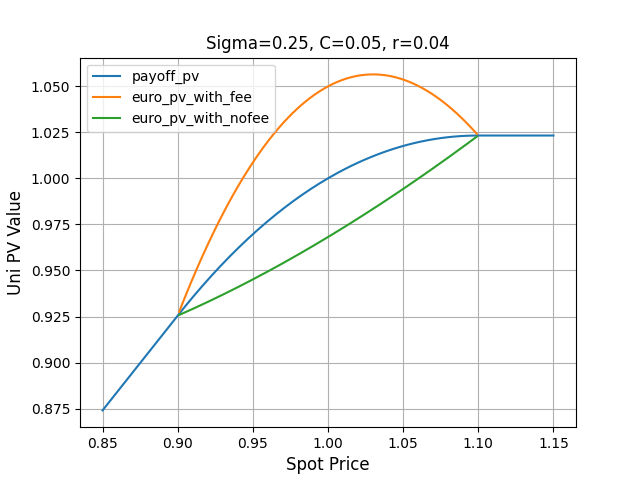
\includegraphics[width=1\linewidth]{figures/euro-pv-spot.png}
    \caption{relation between spot price and present value}
    \label{fig:spot_pv}
\end{figure}
As illustrated in Figure~\ref{fig:spot_pv}, the blue line represents the variation of the payoff pricing model in response to changes in the spot price. The orange and green lines depict the corresponding numerical changes in the pricing model of a European option, where the orange line incorporates transaction costs and discounting, while the green line excludes these factors, both following the fluctuations in the spot price.We can observe that, under the current market parameters, if the option pricing model does not include transaction costs, it results in an expected loss at the current price, meaning that the present value is less than 1.Only by incorporating the potential transaction costs and their discounted value can we generate a positive return.


\section{Sensitivity Analysis}
% 或许换个标题
In the previous sections, we derived the analytical solution of Uniswap V3 positions. In this section, we focus on the sensitivity analysis of the Uniswap V3 position, specifically examining the Greeks associated with a typical European option framework. We previously derived the closed-form solutions for the pricing mechanisms of Uniswap V3 positions. Here, we extend our analysis to assess how variations in underlying parameters affect the pricing—commonly referred to as "Greeks."

\begin{table}[htbp] \caption{$C= 0.2$   $r= 0.05$  $\sigma= 0.7$} \centering \begin{tabular}{|c|c|c|c|c|c|} \hline \textbf{Model} & \textbf{PV} & \textbf{Delta} & \textbf{Gamma} & \textbf{Vega} & \textbf{Rho} \\ \hline Payoff & 1.000 & 0.561 & -0.632 & nan & nan \\ European & 1.422 & 0.427 & -0.747 & 1.720 & -25.892 \\ American & 1.696 & 0.539 & -0.989 & 0.843 & -19.425 \\ \hline
\end{tabular} 
\label{good market condition}
\end{table}



\begin{table}[htbp] \caption{$C= 0.04$  $r= 0.05$  $\sigma= 0.4$} \centering \begin{tabular}{|c|c|c|c|c|c|} \hline \textbf{Model} & \textbf{PV} & \textbf{Delta} & \textbf{Gamma} & \textbf{Vega} & \textbf{Rho} \\ \hline Payoff & 1.000 & 0.784 & -0.883 & nan & nan \\ European & 0.643 & 0.074 & 0.073 & 1.296 & -7.546 \\ American & 1.018 & 0.765 & -1.059 & 0.200 & -2.019 \\ \hline \end{tabular} 
\label{bad market condition}
\end{table}

\begin{figure}
    \centering
    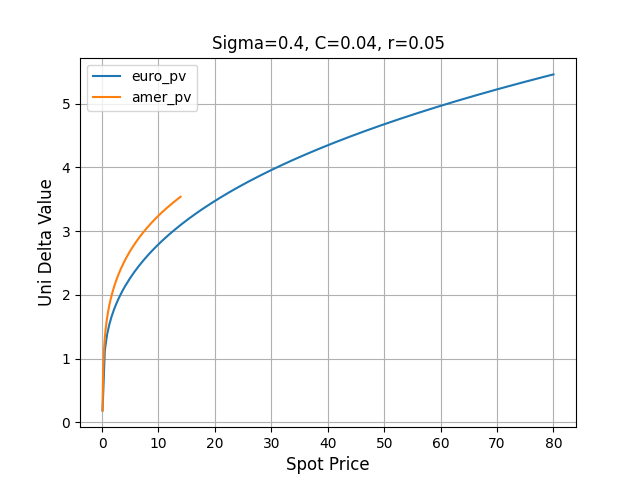
\includegraphics[width=1\linewidth]{figures/good-market-situation-plot.png}
    \caption{Table I market condition pv plot}
    \label{fig:good market situation plot}
\end{figure}

\begin{figure}
    \centering
    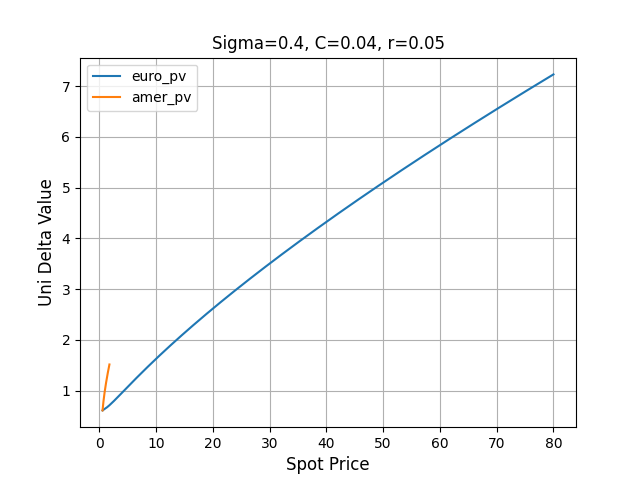
\includegraphics[width=1\linewidth]{figures/bad-market-situation-plot.png}
    \caption{Table II market condition pv plot}
    \label{fig:bad market situation plot}
\end{figure}



\subsection{European and American Present Value Comparison}
We sampled two sets of market parameters based on actual market conditions to observe how the European and American pricing models reflect the actual value of Uniswap range order positions. As illustrated in Table~\ref{bad market condition}, Through numerical analysis, it can be observed that under the market parameters (C=0.04, r=0.05, $\sigma$=0.4), if we immediately establish a Uniswap range order position and exit the position only when it touches the boundary (i.e., behavior under European LP pricing), the present value of such a product will certainly be less than 1. In contrast, if we are able to exit at the optimal execution boundary before reaching the designated boundary, even without achieving a high value of C, we may still obtain a positive return. This is because the American LP pricing model indicates that if a better execution exit boundary exists outside the set LH, a positive return expectation is possible. Furthermore, when C increases (e.g., C=0.2, r=0.05, $\sigma$=0.7), As illustrated in Table~\ref{good market condition}, even with a high value of $\sigma$ (which implies that we may reach the boundary and exit the position more quickly), the European LP pricing model still yields a positive expected value under the current spot price of 1. 
We also plotted the PV-spot graphs for both European and American pricing models under two sets of market parameters. Figures~\ref{fig:good market situation plot} and Figures~\ref{fig:bad market situation plot} clearly demonstrate that, although the early exit boundary for the American option pricing model is narrower, it yields a significantly higher positive expected return compared to the European pricing model.


\begin{figure}
    \centering
    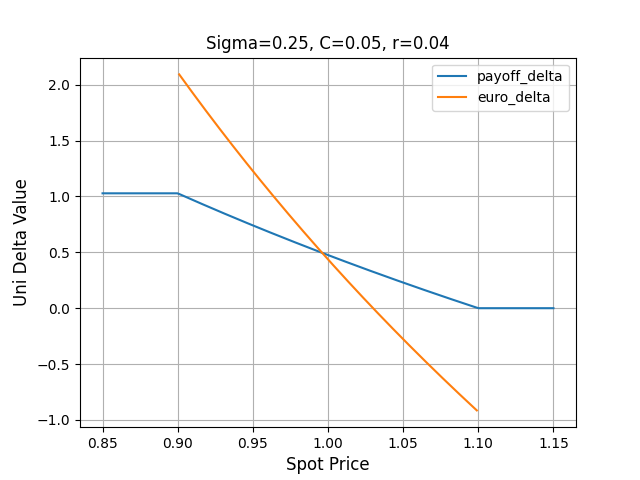
\includegraphics[width=1\linewidth]{figures/differentmodel-delta.png}
    \caption{delta comparison between european and payoff}
    \label{fig:spot_delta}
\end{figure}


\subsection{Delta Analysis}
Delta refers to the sensitivity of the option's price with respect to changes in the underlying asset's price.
As illustrated in Figure~\ref{fig:spot_delta}, the delta for European pricing and payoff valuation reveals noteworthy disparities due to inherent market parameters (C=0.05, r=0.04, $\sigma$=0.25).
 At the orange line's zero point, corresponding to the range (1, 1.05) in the previous analysis, the delta suggests that during actual trading, the delta derived from payoff valuation might lead to residual risks characterized by the Greek value. This indicates potential risk exposure when delta hedging is performed under the assumption of risk neutrality.


\begin{figure}
    \centering
    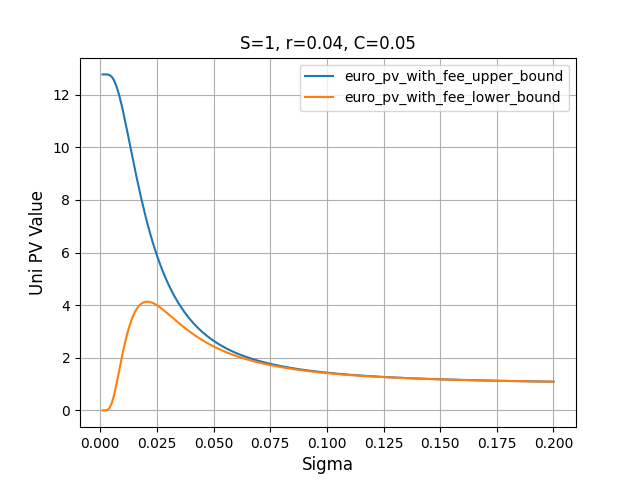
\includegraphics[width=1\linewidth]{figures/different-rebate-cal-method-comparison.png}
    \caption{relation between pv and $\sigma$ using different rebate calculation}
    \label{fig:rebate_comparison}
\end{figure}


\subsection{The Impact of Volatility}
The relationship between the volatility of the underlying asset and the pricing dynamics of the Uniswap V3 position is integral to our sensitivity analysis. Intuitively, we understand that according to the European option valuation model, the present value (PV) pricing should exhibit a monotonically negative correlation with volatility. This stems from the Automatic Market Maker (AMM) mechanism of Uniswap V3, which fundamentally behaves as a short volatility strategy. As the volatility increases, we anticipate a decrease in the valuation, signifying an inverse correlation.

However, the observed orange line in Figure~\ref{fig:rebate_comparison}deviates from this predicted relationship due to the dual pricing model for transaction fees, which has separate methodologies for calculating both upper and lower bounds. The rationale behind the lower bound is driven by the expectation of time until a transaction fee is collected, conceptualized through the theory of stopping times, which is directly proportional to volatility. Conversely, the upper bound assumes continuous trading throughout the transactional process, operating under the premise that serial transactions yield continuous fees, justifying the positive valuation associated with low volatility events.

We selected points with relatively low volatility, such as $\sigma$=0.02, to compare the pricing models of the two transaction fee calculation methods in terms of their present value (PV), as shown in Figure~\ref{fig:different_fee_pv}. In the PV-spot graph, the pricing model based on the upper bound of transaction fees consistently yields a higher value than the pricing model based on the lower bound of transaction fees.


\begin{figure}
    \centering
    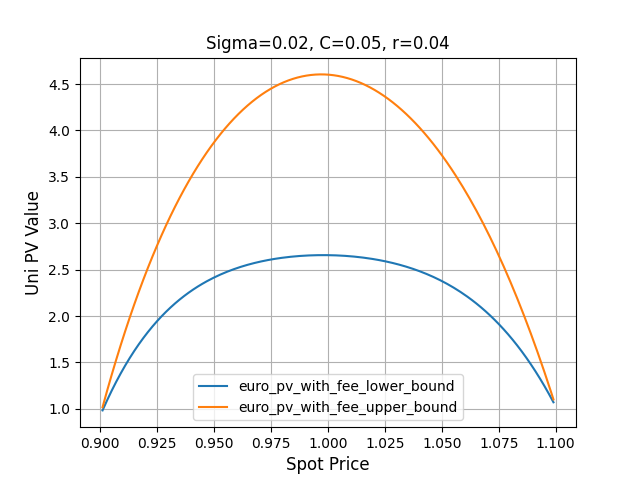
\includegraphics[width=1\linewidth]{figures/differentfee-pv.png}
    \caption{relationship of pv-spot with different fee calculation}
    \label{fig:different_fee_pv}
\end{figure}


\section{future work}
\subsubsection{Hedging Strategies}
Our pricing model is equipped to offer more accurate calculations of Greek risk measures such as delta, gamma, and vega. These calculations are crucial for developing sophisticated hedging strategies. By leveraging these measures, we can devise fully hedged strategies that maximize profitability while minimizing risk. Such strategies will not only benefit LPs by enhancing their returns and reducing risk but also contribute to the overall stability and efficiency of the DeFi ecosystem.

\subsubsection{Adaptation to Uniswap v4}
With the introduction of Uniswap v4, various new decentralized exchange (DEX) paradigms will be implemented, such as dynamic fee structures \cite{b7}, which make \(C\) a function of volatility. This simplification of the model allows LPs to adjust their positions less frequently in response to market conditions, making participation more accessible and efficient. Beyond dynamic fees, many potential enhancements and new models may emerge with Uniswap v4, requiring further adaptations and improvements to our frameworks.

\subsubsection{Implied volatility }
Our model is not only applicable for pricing but also serves as a tool for estimating implied volatility. Similar to the Black-Scholes-Merton (BSM) framework, we can infer the views of LPs on volatility through their positions. By aggregating these inferred volatilities, we can construct a liquidity surface that reflects the weighted perspectives of LPs.


\begin{thebibliography}{00}
\bibitem{b1} H. Adams, N. Robinson, D. Salem, and M. Zinsmeister, "Uniswap v3 Core," Uniswap Labs, 2021,https://app.uniswap.org/whitepaper-v3.pdf

.
\bibitem{b2} G. Lambert, H. Esqueda, and S. Tang, ``Risk-Adjusted Pricing Models for Uniswap V3,'' arXiv, Aug. 2022. [Online]. Available: https://arxiv.org/pdf/2208.06046
\bibitem{b3} G. Lambert, ``Uniswap v3 LP Tokens as Perpetual Put and Call Options,'' Medium, Nov. 2021. [Online]. Available: https://lambert-guillaume.medium.com/uniswap-v3-lp-tokens-as-perpetual-put-and-call-options-5b66219db827

\bibitem{b4} G. Lambert, ``A Guide for Choosing Optimal Uniswap v3 LP Positions, Part 1,'' Medium, Nov. 2021. [Online]. Available: https://lambert-guillaume.medium.com/a-guide-for-choosing-optimal-uniswap-v3-lp-positions-part-1-842b470d2261
\bibitem{b5} D. A. Darling, A. J. F. Siegert "The First Passage Problem for a Continuous Markov Process," The Annals of Mathematical Statistics, Ann. Math. Statist. 24(4), 624-639, (December, 1953)
\bibitem{b6} Shreve, S.E. (2004) Stochastic Calculus for Finance II Continuous-Time Models. Springer, Berlin.
https://doi.org/10.1007/978-1-4757-4296-1
\bibitem{b7} Andrei N. Borodin, Paavo Salminen (2002) Handbook of Brownian Motion - Facts and Formulae. Springer. https://link.springer.com/book/10.1007/978-3-0348-8163-0
\bibitem{b8} Uniswap, ``Volatility Fee Hook,'' Uniswap Documentation, 2024. [Online]. Available: https://docs.uniswap.org/contracts/v4/guides/hooks/Volatility-fee-hook. [Accessed: 13-Nov-2024].
\end{thebibliography}
\vspace{12pt}

\end{document}
